\section{Testes}
	
	A operação da aplicação ARHydra está diretamente relacionada ao tempo que esta necessita para levar a informação ao 
	seu usuário. Com o objetivo de medir este tempo foram realizados testes onde se variou a distância do marcador 
	bem como o equipamento utilizado. Os dados foram analisados com relação a execução completa dos três componentes 
	envolvidos na operação (reconhecimento, decodificação e apresentação). Estes testes foram realizados no ambiente do 
	LAICO (LAboratorio de Sistemas Integrados e COncorrentes), situado no Departamento de Ciências da Computação da 
	Universidade de Brasília. Foram utilizados dois~\textit{smartphones} distintos, um Motorola Defy e um 
	Sansung Galaxy SIII, de forma a avaliar a influência da qualidade da câmera e do processamento durante o uso. O Motorola 
	Defy possui as seguintes especificações: processador Cortex-A8 de 800 MHz, 512 MB de memória RAM, resolução de tela 
	de 480 x 854~\textit{pixels}, GPU (\textit{Graphics Processing Unit}) PowerVR SGX530 e câmera com resolução de 5MP. 
	O Sistema Operacional testado nesse dispositivo foi o Android 2.3.7 com~\textit{firmware} CyanogenMod 7.2. Já o 
	\textit{smartphone} Samsung Galaxy SIII possui processador Quad-core 1.4 GHz Cortex-A9, 1GB de memória RAM, 
	resolução da tela de 720 x 1280~\textit{pixels}, GPU Mali-400MP, câmera com resolução de 8MP e sistema operacional 
	Android 4.0.4.

\subsection{Reconhecimento dos marcadores}
	
	Foram executados conjuntos de testes com o objetivo de mensurar o tempo gasto no processo de
	reconhecimento do marcador proposto. O tempo de reconhecimento é composto pela soma dos tempos gasto
	na identificação das bordas do marcador, do processo de decodificação do QRCode, da obtenção dos
	dados (via integração com a Hydra) referentes ao marcador selecionado e da apresentação dos
	recursos ao usuário. Deste modo, foram propostos testes que realizassem as seguintes medições:
		
	\begin{enumerate}
	  \item \textbf{Medição do tempo do primeiro reconhecimento:} Tempo com que o
	  		marcador é reconhecido pela primeira vez após a aplicação ARHydra ser inicializada;
	  
	  \item \textbf{Medição do tempo de recorrência:} Tempo com que a aplicação gasta para
	  		reconhecer um marcador de forma recorrente, conforme a câmera é movimentada sem que a mesma
	  		perca a visualização do marcador;
	  
	  \item \textbf{Medição do tempo de reconhecimento após o marcador não estar mais no campo de visão da
	  		câmera do \textit{smartphone}:} Tempo médio necessário para que a aplicação
	  		reconheça um novo marcador após o usuário perder o campo de visão do marcador
	  		no~\textit{smartphone}.
	  		
	  \item \textbf{Taxa de erros:} Este valor representa o percentual das ocorrências com que a
			aplicação ARHydra deixou de identificar o marcador quando este estava sendo capturado pela câmera
			do~\textit{smartphone}.
	   
	   \item \textbf{Taxa de não decodificação:} Este valor representa a porcentagem média de falha nas decodificações 
	   		do QRCode inseridos no marcador. As ocorrências nesta taxa são contabilizadas quando um marcador é reconhecido
	   		porém não é feita a decodificação do QRCode pelo Módulo de Decodificação. Esse valor varia de acordo 
	   		com a aplicação responsável pela decodificação, o nível de tolerância a falhas utilizada no QRCode, a 
	   		qualidade da obtenção das imagens pelo dispositivo e a distância entre o marcador e o~\textit{smartphone}. 
	
	\end{enumerate}
	
	A aplicação ARHydra oferece suporte, presente no Módulo de Decodificação, para a utilização de diversos 
	aplicativos ao qual disponibilizem o recurso de decodificação de QRCode's. Através desse suporte foram 
	realizados testes que permitiram estabelecer um comparativo de desempenho entre essas diversas aplicações 
	utilizadas. A fim de obter esse comparativo, as aplicações ZBar~\cite{zbar} e ZXing~\cite{zxing} foram	
	utilizadas nos referidos testes.
	
	Uma outra informação importante a ser definida refere-se ao estabelecimento de uma distância máxima
	para o reconhecimento destes marcadores. Este valor pode variar de acordo com a aplicação
	utilizada no processo de decodificação, considerando as limitações envolvidas no recolhimento das
	informações necessárias para a decodificação mesmo quando os QRCode's apresentarem níveis de
	tolerância a falhas. Desta maneira, para o estabelecimento desse valor, os testes propostos foram
	executados para diferentes distâncias.
	
	As taxas de erros e de não decodificação estão diretamente relacionadas a qualidade da imagem obtida. No entanto,
	esta qualidade não diz respeito somente a resolução da câmera utilizada, outros fatores podem influenciar no
	reconhecimento do marcador. Dentre estes pode-se citar a qualidade das lentes e o algoritmo utilizado na compressão 
	das imagens, possibilitando que seja obtido resultados diferentes para cenários semelhantes, quando estes 
	resultados são coletados utilizando dispositivos dotados de diferentes câmeras. Um outro ponto importante 
	para se garantir esta qualidade está no controle de luminosidade implementado pelas câmeras. Para minimizar esses 
	problemas apresentados é possível ser implementado etapas de pré-processamento da imagem para melhorar a qualidade
	dessa imagem obtida.
	
\subsubsection{Especificações do Marcador}

	O marcador foi construído baseando nas especificações apresentadas pelo QRCode
	(seção~\ref{sec:simbolos_bidimensionais}) e nas dimensões necessárias voltadas para o módulo de
	reconhecimento validar o marcador. Também deve ser considerado a inserção desses marcadores no ambiente de forma menos
	intrusiva possível, mas que suas caraterísticas possibilitem seu reconhecimento.
	
	A Figura~\ref{fig:dimensoes_marcador} apresenta as dimensões adotadas na construção desses
	marcadores. O QRCode é envolvido por uma moldura, com bordas no valor experimental de 0,8 centímetros, 
	para que o módulo de reconhecimento consiga validar e estabelecer as informações de
	posicionamento referentes ao marcador e o módulo de decodificação realize com sucesso a decodificação
	do QRCode.
	
	\begin{figure}[htb]
		\centering 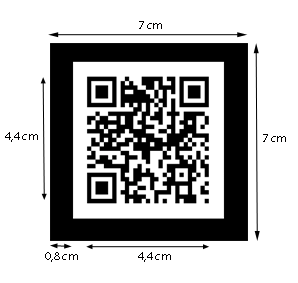
\includegraphics[scale=0.8]{figuras/cap4/dimensoes_marcador.png}
		\caption{\textit{Dimensões do marcador.}}
		\label{fig:dimensoes_marcador} 
	\end{figure}
	
\subsection{Resultados}
\label{sec:resultados}

	Os conjuntos de testes foram executados a uma distância inicial de 50
	centímetros, referente a distância entre o marcador e a aplicação ARHydra executada
	no~\textit{smartphone}, sendo esta aumentada gradativamente em 10 centímetros até atingir o valor 
	de 1 metro. Foram executados os seguintes testes:
	
	\begin{itemize}
	  \item Desempenho e qualidade da obtenção da imagem: Neste teste foi utilizado dois
	  		~\textit{smartphones} com o propósito de estabelecer a diferença de desempenho da aplicação
	  		ARHydra, bem como apresentar o comparativo entre taxas de reconhecimento e não decodificação 
	  		do QRCode para cada~\textit{smartphone} utilizado.
	  
	  \item Suporte a diversas aplicações de decodificação do QRCode: Neste teste foi validado o suporte 
	  		oferecido pela ARHydra para a utilização de diversos aplicativos cujo propósito seja a 
	  		decodificação de QRCodes.
	  		
	  \item Influência da tolerância a falhas do QRCode: Este permite medir a influência dos níveis de 
	  		tolerância a falhas aplicados ao QRCode e sua relação com a taxa de não decodificação.
	  			  
	\end{itemize}

\subsubsection{Teste de desempenho e qualidade na obtenção da imagem}
\label{sec:testesDesempenho}

 
	Um dos objetivos para este teste é comparar o desempenho da aplicação ARHydra utilizada nos dispositivos mencionados 
	anteriormente, com o propósito de  mensurar a diferença nos tempos de reconhecimento do marcador, sendo esta 
	influenciada diretamente pela capacidade de processamento, processador e~\textit{GPU}, de cada dispositivo. O outro 
	objetivo consiste em analisar a influência da qualidade da imagem obtida pela câmera, destes dispositivos, estabelecendo 
	um comparativo entre as taxas de erro e não decodificação.
	
	Para a execução do teste foram realizadas vinte medições para a primeira aparição, duzentas medições para as recorrências 
	e cinquenta medições para o reconhecimento ao perder o marcador. Os resultados dessas medições são apresentados nos 
	gráficos das Figuras~\ref{fig:testeCompDesempenho} e \ref{fig:testeCompTaxas}.
	
	\begin{figure}[htb] 
		\centering 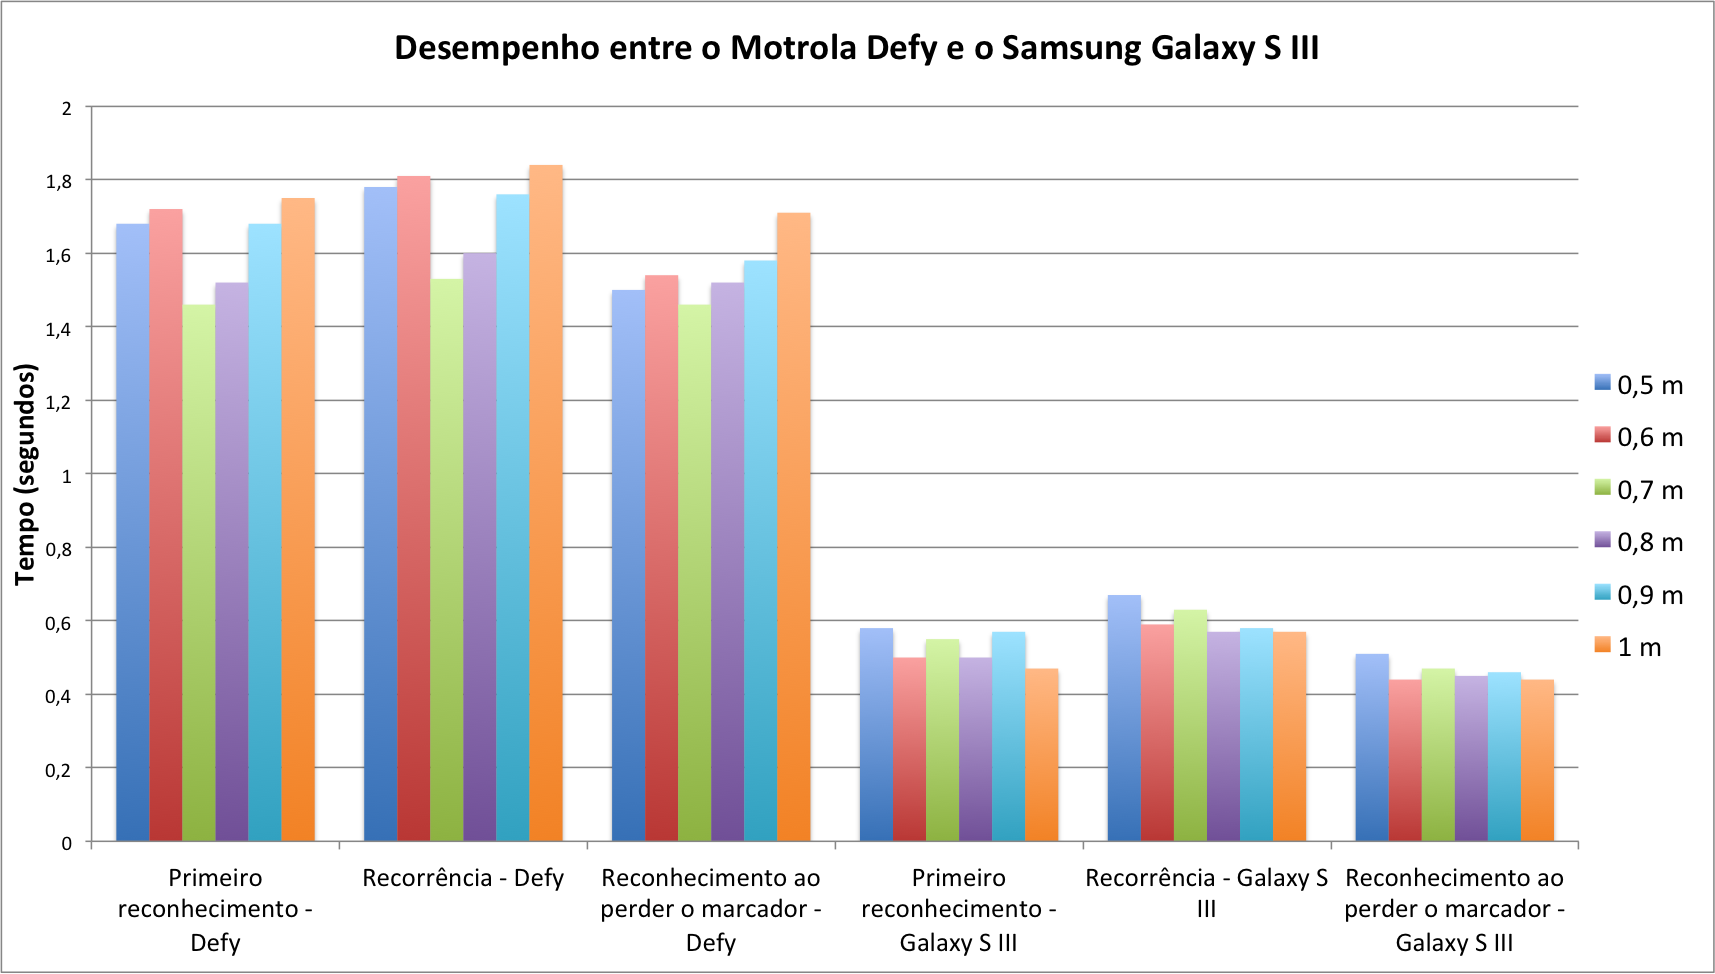
\includegraphics[scale=0.55]{figuras/cap4/grafico_desempenho.png}
		\caption{\textit{Comparativo de desempenho da aplicação ARHydra entre os dispositivos Motorola Defy e 
							Samsung Galaxy SIII.}}
		\label{fig:testeCompDesempenho} 
	\end{figure}
	
	
	A Figura \ref{fig:testeCompDesempenho} apresenta o resultado que mede o desempenho dos dispositivos. Ela mostra que o 
	dispositivo Galaxy SIII obteve melhor desempenho, sendo mais rápido no reconhecimento dos marcadores, devido a diferença 
	na capacidade de processamento, processador e~\textit{GPU}, presente no processador do Galaxy SIII. Desta forma, 
	quanto maior for a capacidade de processamento do dispositivo menor será o tempo gasto pela aplicação ARHydra reconhecer
	os marcadores.   
	
	Os tempos obtidos no primeiro reconhecimento foram inferiores quando comparados ao tempo gasto na recorrência, em ambos 
	os dispositivos, por causa da baixa quantidade de imagens a serem processadas ou descartadas pelos módulos de 
	reconhecimento,	decodificação e apresentação após a captura das imagens ser inicializada. Adicionalmente, a 
	aplicação ARHydra não apresenta um mecanismo de histórico de reconhecimentos ocasionando com que cada 
	reconhecimento concluído com sucesso seja considerado um novo reconhecimento, onerando assim o tempo de recorrência. 
	
	\begin{figure}[htb] 
		\centering 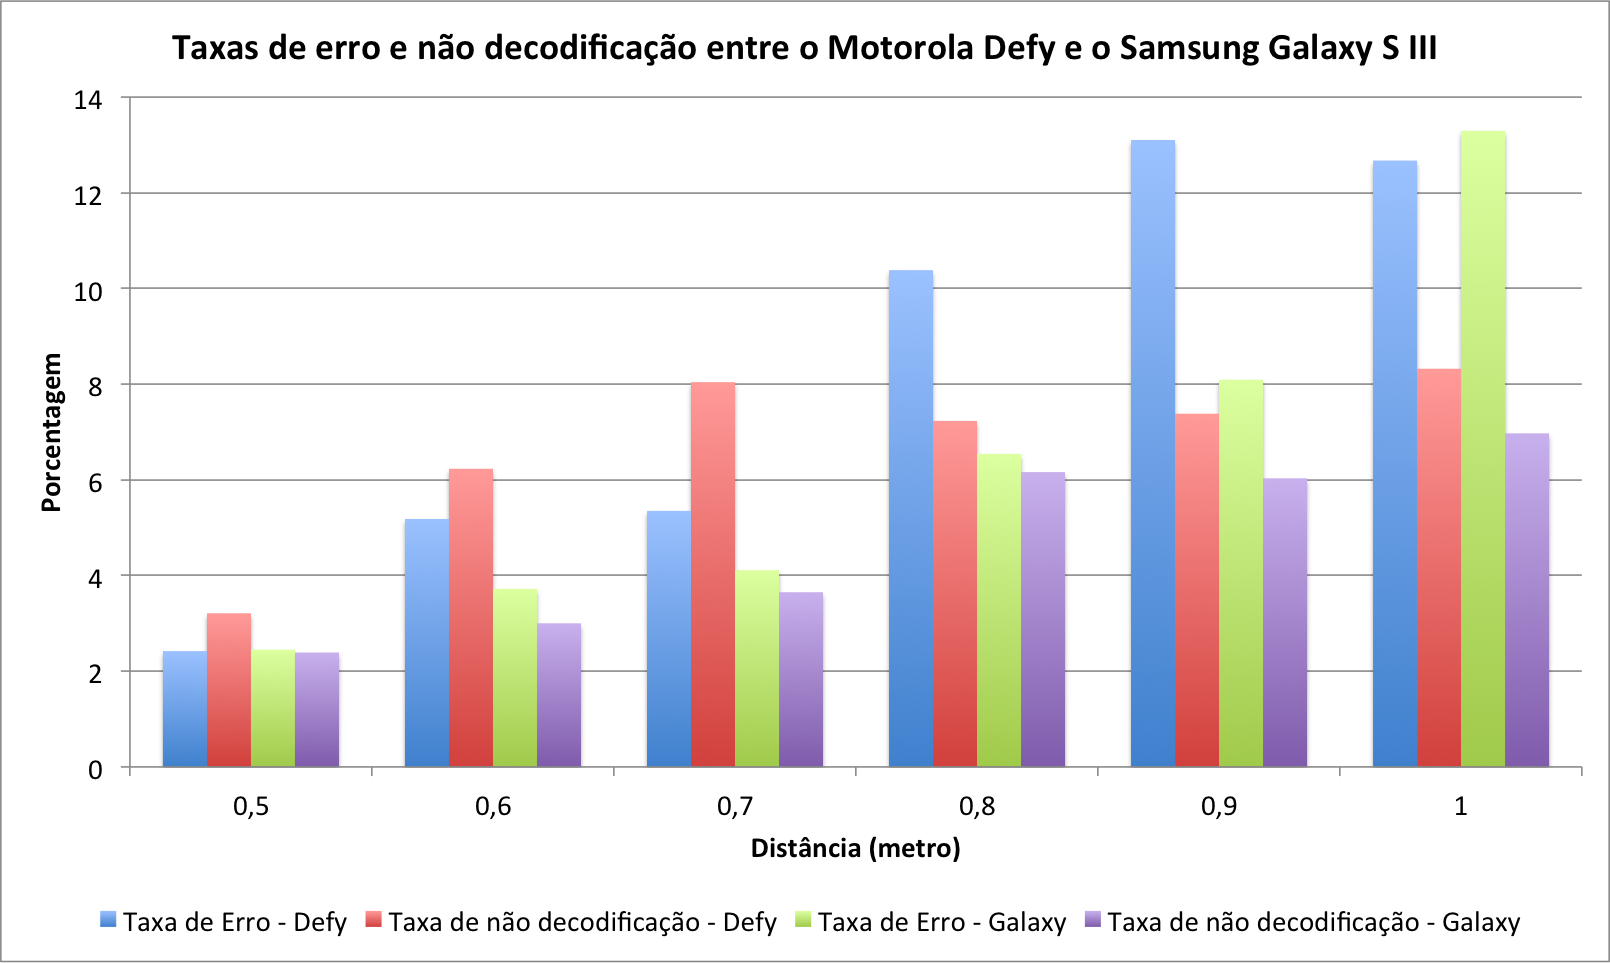
\includegraphics[scale=0.55]{figuras/cap4/grafico_taxas_defy_s3.png}
		\caption{\textit{Comparativo entre as taxas de erro e de não decodificação da aplicação ARHydra entre os 
						dispositivos Motorola Defy e Samsung Galaxy SIII.}}
		\label{fig:testeCompTaxas} 
	\end{figure}
	
	A Figura~\ref{fig:testeCompTaxas} apresenta as Taxa de Erros e Taxa de não decodificação. Novamente o Galaxy SIII 
	mostrou superioridade na maioria das distâncias avaliadas. Esses resultados demonstram a influência da qualidade 
	da imagem capturada em relação as taxas aqui apresentadas. Não levando em consideração as etapas voltadas ao 
	pré-processamento de imagens que possam ser implementadas na ARHydra, conclui-se então que quanto maior for a qualidade da 
	câmera (resolução, qualidade das lentes, algoritmo utilizado na compressão das imagens, controle de luminosidade, etc), 
	juntamente com a melhoria na qualidade dos valores recebidos pelo sensor de orientação do~\textit{smartphone}, menores 
	serão as taxas de erro e decodificação apresentadas na ARHydra. 
	
\subsubsection{Suporte a diversas aplicações de decodificação do QRCode}

	A ARHydra permite a integração de diferentes mecanismos para a decodificação de QRCodes a serem utilizados no Módulo 
	de decodificação. Na atual versão da aplicação é permitido utilizar tanto a implementação fornecida pelo ZBar e o 
	ZXing para esta tarefa. Tomando esta flexibilidade como base, foram realizados testes para verificar o comportamento 
	fornecido por cada um destes. 
	
	Para estes testes foi utilizado o~\textit{smartphone} de melhor capacidade, o Samsung Galaxy SIII, de forma que o 
	nível de tolerância a falhas do QRCode foi ajustado para o modo~\textit{Quality}. Neste teste 
	foram obtidas quinhentas medições por posição em cada implementação. Os resultados obtidos podem ser observados na 
	Figura~\ref{fig:testeSuporte}.
	
	\begin{figure}[htb] 
		\centering 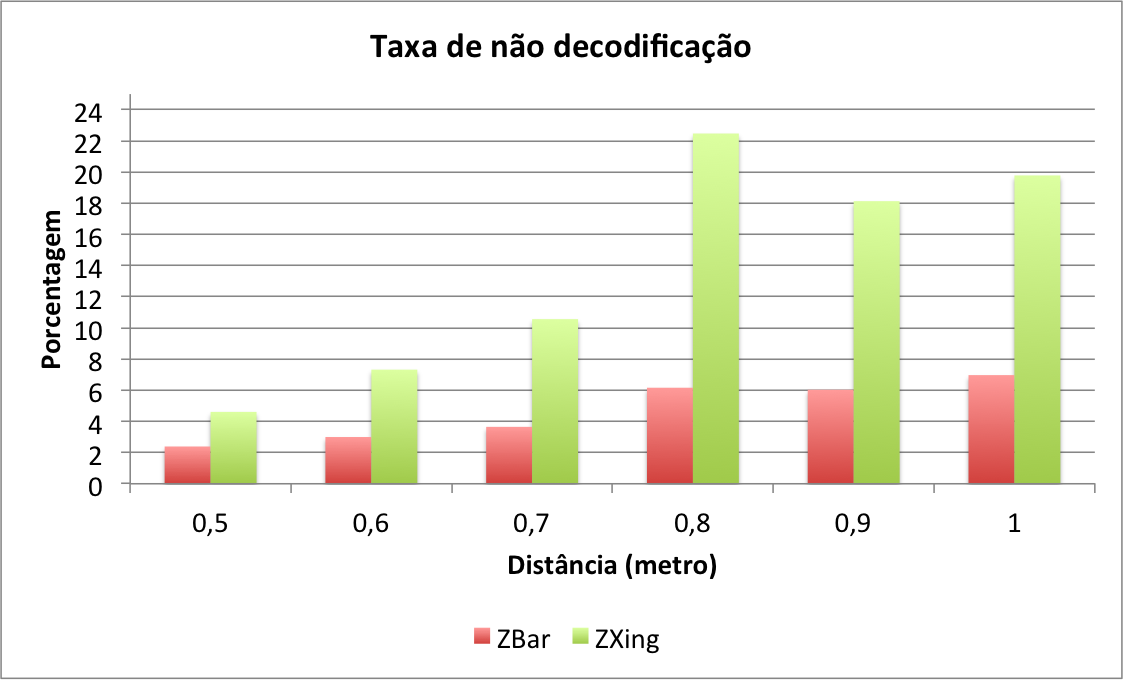
\includegraphics[scale=0.75]{figuras/cap4/grafico_suporte.png}
		\caption{\textit{Taxa de não decodificação para as aplicações ZBar e ZXing.}}
		\label{fig:testeSuporte} 
	\end{figure}
	
	Os resultados apresentados indicam que a implementação ZBar apresenta taxas de não decodificação mais baixas do 
	que a ZXing. Na maioria das distâncias analisadas, ambas as aplicações apresentaram aumento em suas taxas a 
	medida com que a distância fosse aumentada. A diferença apresentada nos resultados está relacionado ao algoritmo 
	utilizado por essas aplicações, porém não foi possível obter informações a respeito da implementação dos mesmos.
	
	
\subsubsection{Influência da tolerância a falhas do QRCode}

	%Estes níveis tem por objetivo facilitar a decodificação do QRCode, porém o formato do 
	%local de armazenamento de seu conteúdo varia de acordo com seu nível de tolerância a falhas implementado.
	
	Como visto na seção \ref{sec:simbolos_bidimensionais}, os QRCodes podem ser compostos por quatro níveis de 
	tolerância a falhas. Este conjunto de testes por sua vez, visa estabelecer um parâmetro de qual nível seria 
	melhor aplicado à aplicação ARHydra, uma vez que a longa distâncias a câmera não consegue capturar os pontos 
	do QRCode, impossibilitando	assim sua decodificação. 
	
	Para análise dos resultados foram realizadas quinhentas medições para cada distância, sendo esta 
	repetida para todos os níveis de tolerância a falhas. Por fim, o módulo de decodificação foi configurado 
	para utilizar a	aplicação ZBar nos testes mencionados, devido suas melhores taxas obtidas no teste anterior. 
	
	\begin{figure}[htb]
		\centering 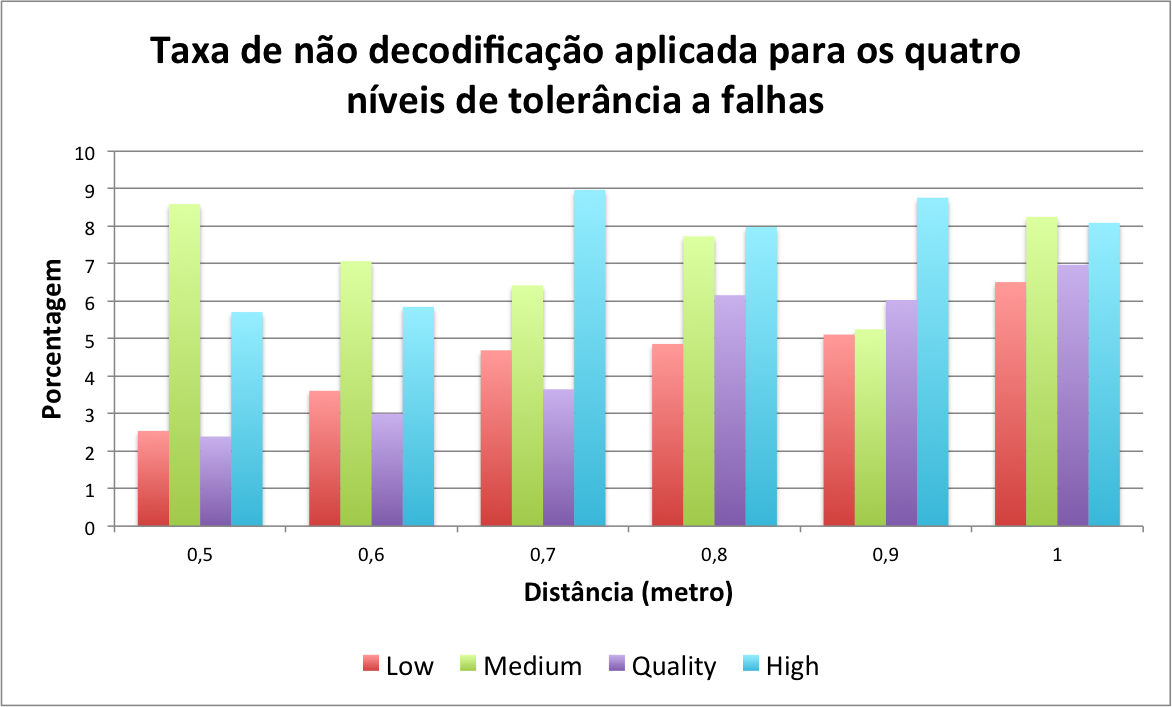
\includegraphics[scale=0.75]{figuras/cap4/grafico_nivel_decode.png}
		\caption{\textit{Nível da taxa de não decodificação aplicado sobre a influ{\^e}ncia da toler{\^a}ncia a falhas do QRCode.}}
		\label{fig:testeNivelDecode} 
	\end{figure}
	
	A Figura \ref{fig:testeNivelDecode} apresenta os resultados para este teste. Estes níveis possuem percentuais de 
	recuperação a falhas conforme a Tabela~\ref{tab:nivelFalha}. Os marcadores, quando ajustados aos 
	níveis~\textit{Low} e~\textit{Quality}, obtiveram melhores resultados comparado aos demais níveis. Embora, as taxas 
	de todos os níveis tenham apresentado aumento à medida que o dispositivo se afastava do marcador em questão. Quando 
	os níveis~\textit{Low} e~\textit{Medium} são comparados, é possível observar que o formato de seus campos responsáveis
	pela estruturação do QRCode, mesmo quando a diferença na porcentagem da tolerância a falhas é pequena, interfere na 
	obtenção dos pontos	internos ao código, ocasionando uma variação muito grande na taxa de não decodificação. 
	Esse mesmo comportamento é observado para os níveis~\textit{Quality} e~\textit{High}. 
	
	A medida com que é elevado o nível de tolerância a falhas há um aumento da quantidade de informação a ser armazenada
	para cobrir a porcentagem de informação que pode ser recuperada. No entanto, o espaço ocupado pelo QRCode, no marcador 
	utilizado, permaneceu o mesmo, independente do nível de recuperação a falhas aplicado. Desta forma, quanto maior o nível de 
	recuperação a falhas utilizado mais complexo será a decodificação do marcador utilizado. A partir dos resultados 
	analisados, conclui-se que o nível~\textit{Low} de tolerância a falhas é o que melhor se aplica para utilização na 
	aplicação ARHydra para as distâncias analisadas. 
	
	
	